\subsection{Definition von Emotionen} \label{definition-emotionen}



Der Begriff ``Emotion'' wird zwar weltweit  (in fast allen Sprachen) und von alle Menschen verwendet (die soziale oder intellektuelle Ebene spielt keine Rolle), ist aber relativ schwer zu definieren. 
Dieses Paradox wurde bereits im folgenden Zitat explizit erw{\"a}hnt: 
``Everybody knows what an emotion is, until asked to give a definition.''\cite{fehr_russel_1984} von Fehr und Russell, zwei amerikanischer Emotionsforscher (Psychologe). 
Noch {\"u}berraschender ist die Schwankung in der Definition dieses Begriffs ``Emotion'' im Laufe der Zeit: Allein die englischsprachige Experimentalpsychologie\cite{plamper12} liefert zwischen 1872 und 1980 mehr als 92 verschiedene Definitionen. 
Wir verstehen daher, dass es schwierig w{\"a}re, zu versuchen, diese Definition zu formulieren.  
Wie k{\"o}nnen wir also die Schwierigkeit, eine Definition f{\"u}r einen solchen gemeinsamen Begriff zu finden, erkl{\"a}ren? 
Man sollte nicht vergessen werden, dass es sich um einen eher abstrakten Begriff handelt und daher ist die Emotion sehr subjektiv. 
Neben diesem abstrakten Aspekt ist auch anzumerken, dass sich der Begriff der Emotion auch auf viele Bereiche bezieht, die sich ebenso voneinander unterscheiden wie sie variieren: z.B. Literatur, Philosophie, Psychologie usw. 
Neben diesem multidisziplin{\"a}ren Charakter, der die Pluralit{\"a}t der Vorstellungen und Ans{\"a}tze in jedem Definitionsversuch erkl{\"a}ren k{\"o}nnte, ist es auch notwendig, die Variationen von Sprachen, Perioden und sogar Kulturen hinzuzuf{\"u}gen. \\


Es wird uns allein mit dieser Arbeit (und das ist auch nicht von uns erwartet) nicht m{\"o}glich sein, alle Fragen im Zusammenhang mit der Definition des Begriffs ``Emotion'' zu betrachten, aber wir werden einige konkrete Beispiele vorstellen, um die Komplexit{\"a}t zu veranschaulichen, die sich aus der Suche nach einer Definition von Emotion ergeben kann.  
Die antiken Philosophen\cite{geslin13} waren die ersten, die sich mit Emotionen und ihren Einfl{\"u}ssen auf den Alltag besch{\"a}ftigen haben. 
Tats{\"a}chlich nahmen Stoiker wie Zeno und Plato bereits 370 n. Chr. Emotionen als eine Krankheit der Seele wahr, die f{\"u}r sie ein Hindernis f{\"u}r denjenigen war, der denken wollte. 
Platon geht mit seiner Allegorie von der H{\"o}hle tiefer, indem er alles was emotional ist  mit alle vern{\"u}nftig (verst{\"a}ndlich) kontrastiert: das hei{\ss} Emotion und Vernunft gehen nicht zusammen. 
Descartes und Aristoteles vervollst{\"a}ndigen Platons Beobachtungen, indem sie in die Analyse von Emotionen eine Dualit{\"a}t (positiv und negativ) der Perzeption einbringen. 
Aristoteles glaubt, dass alles, was das Leben auf positive Weise beeinflusst, durch positive Emotionen bedingt ist, und Descartes glaubt, dass Emotionen f{\"u}r unser {\"u}berleben unerl{\"a}sslich sind und dass die Schw{\"a}che eines Menschen eng mit der F{\"a}higkeit der Seele verbunden ist, seine Emotionen zu kontrollieren. 
Charles Darwin in seinem pr{\"a}sentierte weitere ebenso faszinierende neue Elemente {\"u}ber Emotionen, ohne den bisherigen Beobachtungen zu widersprechen\cite{darwin1872}. 
Er verallgemeinert die Emotionen f{\"u}r alle Kulturen und fand sogar {\"a}hnlichkeit mit Tiere. 
Der Darwin pr{\"a}sentiert  Emotionen  als K{\"o}rpersignale (oder Reaktionen) auf {\"a}u{\ss}ere Handlungen(Externe Ereignisse), begleitet von spezifischen k{\"o}rperlichen {\"a}u{\ss}erungen wie: Gesichtsausdr{\"u}cke, Gesten und oft Ger{\"a}usche, die alle  spezifisch je nach Emotionen sind. \\


So k{\"o}nnen wir weiterhin andere ber{\"u}hmte wissenschaftliche Namen wie William James\cite{james1884}, Walter Cannon\cite{cannon32}, Stanley Scharter\cite{schachter59} usw. nennen, die zu unterschiedlichen Zeiten und an unterschiedlichen Orten das Thema untersucht haben, mit ebenso relevanten wie unterschiedlichen Schlussfolgerungen, aber die Beobachtung bleibt die gleiche, die Definition bleibt unbest{\"a}ndig.
Neben den Schwierigkeiten, die sich aus den oben genannten unterschiedlichen Wahrnehmungen ergeben, tr{\"a}gt die  t{\"a}gliche missbr{\"a}uchliche Verwendung bestimmter Begriffe wie Gef{\"u}hl, Affekt, Stimmung, Gef{\"u}hl (um nur einige zu nennen) als Synonym f{\"u}r Emotionen dazu bei  mehr Verwirrung in das Verst{\"a}ndnis von Emotionen. Diese Begriffe beziehen sich zwar auf Gem{\"u}tszust{\"a}nde, sind aber jedoch nicht Synonym von Emotion\cite{plamper12}.
Trotz des fehlenden Konsenses {\"u}ber die Frage der Definition dieses Begriffs gibt es jedoch Elemente, die in allen Definitionsversuchen wiederkehren, n{\"a}mlich: 

\begin{itemize} \setlength\itemsep{-0.15cm}
  \item das Vorhandensein eines Ausl{\"o}sers;
  \item den psychischen Zustand des Subjekts;
  \item einen bestimmten K{\"o}rperausdruck;
  \item eine physiologische Reaktion (Herzfrequenz, Atmung,Schwitzen ...);
  \item eine bestimmte Qualit{\"a}t, Intensit{\"a}t und Dauer.
\end{itemize}


Basierend auf den obigen Elementen k{\"o}nnen wir daher zu dem Schluss kommen, dass wir zwar nicht genau definieren k{\"o}nnen, was eine Emotion ist, k{\"o}nnen wir aber jedoch jede davon mit Bestimmte spezifisch  Element in Verbindung setzen: einen Stimulus (der der Ausl{\"o}ser der Emotion ist), eine physiologische und k{\"o}rperliche Reaktion. 
Die Existenz mehrerer verschiedener Emotionen l{\"a}sst sich gerade wegen der Spezifit{\"a}t dieser Elemente vermuten. 
Im n{\"a}chsten Teil werden wir versuchen, die verschiedenen Emotionen zu klassifizieren, mit einem besonderen Fokus auf diejenigen, die wir zu induzieren versuchen. \\


Wie bei der Definition von Emotionen gibt es keine einheitliche Klassifizierung von Emotionen. 
Und wie bei den versuchten Definitionen gab es im Laufe der Zeit mehrere vorgeschlagene Klassifikationen, die sich auch im Laufe der Zeit entwickelt haben. 
Diese Mehrheit von klassifikationen ist vermutlich eine Folge des Mangels an Konsens {\"u}ber die Definition selbst. 
Es gibt jedoch zwei Arten von Klassifikationen, die vor allem unterscheidet und durchgesetzt haben: eine dimensionale Klassifikation\cite{geslin13} und eine kategorische Klassifikation\cite{basic_emotions_theories}.




\subsubsection{Kategoriale Klassifikation} \label{kategoriale-klassifikation}

Angetrieben von Charles Darwin, (der auch der erste war, der grundlegende Emotionen identifizierte) diese Vorgehensweise ist die von Emotionsforscher  mit einer evolution{\"a}ren Ansatz. 
Diese Klassifikation basiert auf der Existenz von eine Reihe von sogenannten Grundemotionen oder prim{\"a}re Emotionen. 
Diese  Emotionen w{\"a}re in einer begrenzten Anzahl und ihre Entwicklung wurde stark von der Evolution  beeinflusst. 
Wie viele Dinge in Bezug auf die Emotionen in allgemein, variiert die Anzahl von Grundemotionen von einem Emotionsforscher zu einem anderen (siehe Tabelle \ref{vergleich-basisemotionen}).


\begin{table}[h] \centering
\begin{tabular}{| p{5cm} | p{11cm} |}
\hline
\textbf{Forscher} & \textbf{Basisemotionen} \\ \hline
Gray (1982) & Furcht, Freude, {\"a}rger \\ \hline
Panksepp (1982) & Furcht, Erwartung, {\"a}rger, Panik \\  \hline
Tomkins (1984) & Furcht, Freude, {\"a}rger, Verzweiflung, Ekel, {\"u}berraschung, Interesse, Scham, Zufriedenheit \\  \hline
Plutchik (1980) & Furcht, Freude, {\"a}rger, Traurigkeit, Ekel, {\"u}berraschung, Akzeptanz, Erwartung \\  \hline
Arnold (1960) & Furcht, Liebe, {\"a}rger, Traurigkeit, Hass, Hoffnung, Begehren, Mut, Niedergeschlagenheit, Verzweiflung, Widerwille \\  \hline
Oatley \& Johnson-Laird (1987) & Furcht, Gl{\"u}ck, {\"a}rger, Traurigkeit, Ekel \\  \hline
Ekman (1982) & Furcht, Freude, {\"a}rger, Traurigkeit, Ekel, {\"u}berraschung \\  \hline
Izard (1987) & Furcht, Freude, {\"a}rger, Traurigkeit, Ekel, {\"u}berraschung, Interesse,Verachtung \\ \hline
\end{tabular} \caption[Vergleich einige Basisemotions-Theorien]{ Vergleich einige Basisemotions-Theorien\cite{basic_emotions_theories}. } \label{vergleich-basisemotionen}
\end{table}



Obwohl sie sich nicht {\"u}ber die Anzahl der Grundemotionen einig sind, sind sich die Forscher einig {\"u}ber die Existenz komplexerer Emotionen, die die Kombination mehrerer prim{\"a}rer Emotionen w{\"a}ren. 
Basierend auf diesem Ansatz wurden mehrere Theorien entwickelt, um Emotionen darzustellen, von denen eine der bekannte das Plutchik-Modell ist. 
Plutchiks Modell verwendet ein radf{\"o}rmiges Diagramm (siehe Abbildung \ref{plutchik}) und verschiedene Farben, um jede Emotion darzustellen. \\


\begin{figure}[h]
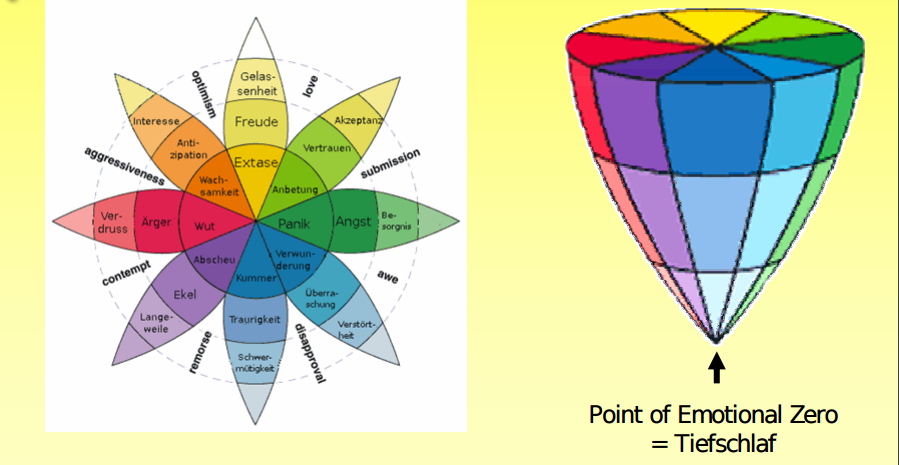
\includegraphics[width=\textwidth]{Images/plutchik.png} 
\vspace{-0.3cm} 
\caption{ Einordnung von Emotion nach Plutchik. }
\label{plutchik} 
\end{figure}


Diese Theorie fundiert sich auf  das acht prim{\"a}re Emotionen mit einer klare trennung (bzw unterschied) zwischen  prim{\"a}ren, sekund{\"a}ren und terti{\"a}ren Emotionen.
Die verbindet jede prim{\"a}re Emotion mit spezifischen Motivationssystem und Verhaltendstedenze zur Bew{\"a}ltigung grundlegender adaptiver Probleme (siehe Tabelle \ref{verhalten-funktion}). 


\begin{table}[h] \centering
\begin{tabular}{| p{5.1cm} | p{5.1cm} | p{5.1cm} |}
\hline
\textbf{Subjektiv} & \textbf{Verhalten} & \textbf{Funktion} \\ \hline
Angst, Entsetzen & R{\"u}ckzug, Flucht  & Schutz \\ \hline
{\"a}rger, Wut & Angriff, Bei{\ss}en & Zerst{\"o}rung \\ \hline
Freude, Ekstase & Paarung, Besitz & ergreifen Fortpflanzung \\ \hline
Traurigkeit, Trauer & Weinen, Bitte um Hilfe & Reintegration \\ \hline
Akzeptanz, Anbetung, Vertrauen & Paarbildung, Pflege & Zusammengeh{\"o}rigkeit, Bindung \\ \hline
Ekel, Abscheu & Sich {\"u}bergeben & Ablehnung, Zur{\"u}ckweisung \\ \hline
Erwartung, Antizipation & Untersuchen & Exploration, Erkundung \\ \hline
{\"u}berraschung & Innehalten, Einfrieren & Orientierung \\ \hline
\end{tabular} \caption[ Einige Basisemotionen jeweils mit Verhalten und Funktio ]{ Einige Basisemotionen jeweils mit Verhalten und Funktion\cite{basic_emotions_theories}. } \label{verhalten-funktion}
\end{table}






\subsubsection{Circumplex Modell} \label{kategoriale-ansatz}

Dieser von Wundt\cite{basic_emotions_theories} initiierte Ansatz geht von dem Gedanken aus, dass die emotionale Erfahrung in einem mehrdimensionalen Raum dargestellt werden kann. 
Dieser Zerlegung der emotionale Erfahrung  sollte es erm{\"o}glichen, eine genaue Analogie zwischen Emotion und K{\"o}rperausdruck (Gesichtsausdr{\"u}cke) herzustellen. 
Dieser Ansatz wurde  daher den Vorteil, dass sie die T{\"u}r zu einer m{\"o}glichen Quantifizierung der emotionalen Erfahrung {\"o}ffnet. 
Die Idee von Wundt (siehe Abbildung \ref{wundt})  war einer dreidimensionalen Zerlegung(Lust-Unlust, Spannung-Entspannung (L{\"o}sung), Beruhigung (Ruhe)-Erregung siehe) der emotionalen Erfahrung. 


\begin{figure}[h]
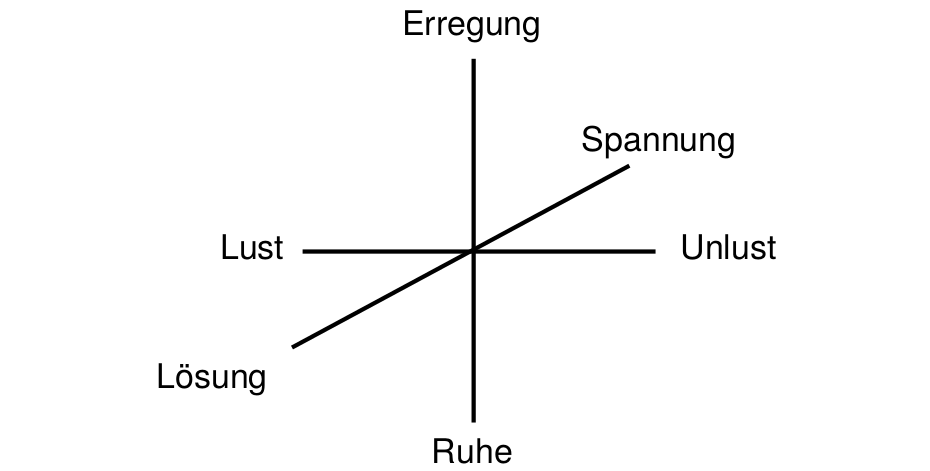
\includegraphics[width=\textwidth]{Images/wundt.png} 
\vspace{-0.3cm} 
\caption[Einordnung von emotionale Erfahrungsprozess nach Wundt.]{ Einordnung von emotionale Erfahrungsprozess nach Wundt\cite{basic_emotions_theories}. }
\label{wundt} 
\end{figure}


Die Frage nach der Anzahl der Dimensionen, die zur Darstellung der emotionalen Erfahrung notwendig sind, wird jedoch zu mehreren Theorien f{\"u}hren. 
Allerdings schlug Russell\cite{basic_emotions_theories} eine zweidimensionale Darstellung mit sechs prim{\"a}ren Emotionen nach Ekam vor (siehe Tabelle \ref{vergleich-basisemotionen}). 
Emotionen werden also dank dieses Modells (siehe Abbildung \ref{russell}) eine horizontale Komponente haben: Valenz (Freude/Verdruss) und eine vertikale Komponente: Erregung (Aktivierung). 


\begin{figure}[h] \centering
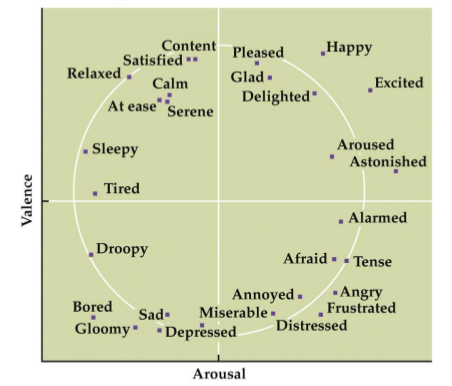
\includegraphics[width=12cm]{Images/russell.png} 
\vspace{-0.3cm} 
\caption[Einordnung von emotional Erfahrung nach Russell.]{ Einordnung von emotional Erfahrung nach Russell\cite{basic_emotions_theories}. }
\label{russell} 
\end{figure}


Die Valenz unterscheidet positive Emotionen von negative Emotionen, und die Erregung informiert {\"u}ber k{\"o}rperliche Erregung, die man durch die Anzahl von physiologischen Reaktion feststellen kann. 
Jede Emotion l{\"a}sst sich als Kombination dieser beiden Parameter darstellen was f{\"u}r eine mathematische auswertung sehr hilfreich sein k{\"o}nnte. 
Dieses Modell hat viel Erfolg gehabt, da er die Darstellung von eine Unendlichkeit von Emotionen erlaubt hat. 
Trotz der unterschiedlichen Anzahl von Dimensionen von verschiedenen Autoren vorgeschlagen, die beiden Dimensionen von Russell (Valenz und Erregung) sind Faktoren die in fast alle Modelle dieses Ansatzes auftreten.



